\section{Results}\label{sec:results}

This chapter compares the results of rule-based trade classification with machine learning-based classification. The results suggest a supremacy of machine learning-based classifiers.

\subsection{Results of Rule-Based Approaches}\label{sec:result-of-rule-based-approaches}

We now estimate the accuracy of classical trade classification rules on the \gls{ISE} and \gls{CBOE} sample. We consider the tick and quote rule, as well as the \gls{LR} algorithm, \gls{EMO} rule and \gls{CLNV} method in their classical and reversed formulation. Additionally, we consider two stacked combinations of \textcite[][12--14]{grauerOptionTradeClassification2022} due to their state-of-the-art performance on the validation set, as derived in \cref{sec:hyperparameter-tuning}. Namely, $\operatorname{quote}_{\mathrm{nbbo}} \to \operatorname{quote}_{\mathrm{ex}} \to \operatorname{rtick}_{\mathrm{all}}$ and $\operatorname{tsize}_{\mathrm{ex}} \to \operatorname{quote}_{\mathrm{nbbo}} \to \operatorname{quote}_{\mathrm{ex}} \to \operatorname{depth}_{\mathrm{nbbo}} \to \operatorname{depth}_{\mathrm{ex}} \to \operatorname{rtick}_{\mathrm{all}}$ or in short $\operatorname{gsu}_{\mathrm{small}}$ and $\operatorname{gsu}_{\mathrm{large}}$.

We report in \cref{tab:ise_supervised_all-master} accuracies for the entire data set and separate subsets spanning the periods of train, validation, and test set as defined in \cref{sec:train-test-split}. Doing so enables comparisons with previous works, but also provides meaningful estimates on the test set relevant for benchmarking purposes.

Our results are approximately similar to \textcite[][29--33]{grauerOptionTradeClassification2022}. Minor deviations exist, which can be pinned down to differences in handling of unclassified trades and non-positive spreads, as well as divergent implementations of the depth rule.\footnote{Correspondence with the author.}

From all rules, the tick rule performs worst when applied to trade prices at the trading venue with accuracies of a random guess, \SI{49.67}{\percent}. For comparison, a simple majority vote achieves \SI{51.40}{\percent} accuracy. The tick test performs best when estimated on the consecutive trade prices, and additionally, when estimated at the inter-exchange level marginally improves over a random classification, achieving accuracies of \SI{55.25}{\percent} for the reversed tick test. Due to the poor performance, of tick-based algorithms at the exchange level, we estimate all hybrids with $\operatorname{tick}_{\mathrm{all}}$ or $\operatorname{rtick}_{\mathrm{all}}$.

\begin{table}[ht]
    \centering
    \caption[Accuracies of Rule-Based Approaches On \glsentryshort{ISE}]{This table shows the accuracy of common trade classification rules and their variations for option trades on \gls{ISE} sample. Unclassifiable trades by the respective rule are assigned randomly as buy or sell. Hybrid methods are estimated using trade prices across all exchanges. We report the percentage of classifiable trades and the overall accuracy for subsets based on our train-test split and the entire dataset. Best rule in \textbf{bold}.}
    \label{tab:ise_supervised_all-master}
    \begin{tabular}{@{}lSSSSS@{}}
        \toprule
        {}                                     & {Coverage in \%}  & \multicolumn{4}{c}{Accuracy in \%}                                                             \\ \cmidrule(lr){2-2} \cmidrule(lr){3-6}
        {Trade Classification Rule}            & {All}             & {Train}                   & {Val}  & {Test}  & {All}             \\\midrule
        $\operatorname{tick}_{\mathrm{ex}}$    & 91.5800           & 49.1842                            & 50.5441           & 50.2394           & 49.6674           \\
        $\operatorname{rtick}_{\mathrm{ex}}$   & 90.3500           & 52.1701                            & 50.3068           & 50.5258           & 51.4682           \\
        $\operatorname{quote}_{\mathrm{ex}}$   & 94.6900           & 66.2659                            & 57.5174           & 56.9997           & 62.6606           \\
        $\operatorname{lr}_{\mathrm{ex}}$      & 99.8800           & 66.1320                            & 57.5550           & 57.0623           & 62.6004           \\
        $\operatorname{rlr}_{\mathrm{ex}}$     & 99.7200           & 66.3858                            & 57.6456           & 57.1372           & 62.7857           \\
        $\operatorname{emo}_{\mathrm{ex}}$     & 98.7300           & 56.5416                            & 53.7133           & 53.7864           & 55.4243           \\
        $\operatorname{remo}_{\mathrm{ex}}$    & 98.9500           & 57.1490                            & 53.6360           & 54.1495           & 55.8459           \\
        $\operatorname{clnv}_{\mathrm{ex}}$    & 98.7000           & 60.1181                            & 55.2305           & 54.7502           & 58.0656           \\
        $\operatorname{rclnv}_{\mathrm{ex}}$   & 95.0000           & 60.8498                            & 55.3888           & 55.0784           & 58.6019           \\ \midrule
        $\operatorname{tick}_{\mathrm{all}}$   & 97.8500           & 52.8954                            & 54.5403           & 53.3412           & 53.3134           \\
        $\operatorname{rtick}_{\mathrm{all}}$  & 96.7000           & 55.9539                            & 54.4020           & 53.9891           & 55.2500           \\ \midrule
        $\operatorname{quote}_{\mathrm{nbbo}}$ & 99.8900           & 66.8153                            & 58.5520           & 59.5565           & 63.7093           \\
        $\operatorname{lr}_{\mathrm{nbbo}}$    & 99.7900           & 66.6404                            & 58.5902           & 59.6145           & 63.6236           \\
        $\operatorname{rlr}_{\mathrm{nbbo}}$   & 98.7200           & 66.8250                            & 58.6446           & 59.6458           & 63.7515           \\
        $\operatorname{emo}_{\mathrm{nbbo}}$   & 98.3900           & 58.2850                            & 54.8106           & 55.9278           & 57.1183           \\
        $\operatorname{remo}_{\mathrm{nbbo}}$  & 98.9000           & 58.9415                            & 54.8198           & 56.2168           & 57.5718           \\
        $\operatorname{clnv}_{\mathrm{nbbo}}$  & 98.9000           & 61.5439                            & 56.3371           & 57.0753           & 59.6079           \\
        $\operatorname{rclnv}_{\mathrm{nbbo}}$ & 98.7000           & 62.2628                            & 56.5928           & 57.4307           & 60.1614           \\ \midrule
        $\operatorname{gsu}_{\mathrm{small}}$  & 99.8400           & 66.7098                            & 58.7642           & 59.8383           & 63.7449           \\
        $\operatorname{gsu}_{\mathrm{large}}$  & \bfseries 100.000 & \bfseries 79.7126                  & \bfseries 68.8358 & \bfseries 67.2039 & \bfseries 75.0322 \\
        \bottomrule
    \end{tabular}
\end{table}

\todo{How can the coverage of the gsu method be smaller than quote nbbo alone?}

Quote-based algorithms outperform tick-based algorithms delivering accuracy up to \SI{63.71}{\percent}, when estimated on the \gls{NBBO}. The superiority of quote-based algorithms in option trade classification has previously been documented in \textcites{savickasInferringDirectionOption2003}{grauerOptionTradeClassification2022}.

The performance of hybrids, such as the \gls{LR} algorithm, hinges on the reliance on the tick test. Thus, the \gls{EMO} rules and to a lesser extent the \gls{CLNV} rules perform worst, achieving accuracies between \SI{55.42}{\percent} and \SI{57.57}{\percent}. In turn, variants of the \gls{LR}, which uses the quote rule for most trades, are among the best-performing algorithms. By extension, $\operatorname{gsu}_{\mathrm{small}}$ further reduces the dependence on tick-based methods through the successive applications of quote rules, here $\operatorname{quote}_{\mathrm{nbbo}} \to \operatorname{quote}_{\mathrm{ex}}$.

Notably, $\operatorname{gsu}_{\mathrm{large}}$, the combination of \textcite[][33]{grauerOptionTradeClassification2022} including overrides from the trade size and depth rules performs best, achieving \SI{67.20}{\percent} accuracy on the \gls{ISE} test set and \SI{75.03}{\percent} on the entire dataset. Yet, the performance deteriorates most sharply between sets, as visualised in \cref{fig:classical-accuracies-over-time}.

\begin{figure}[ht]
    \centering
    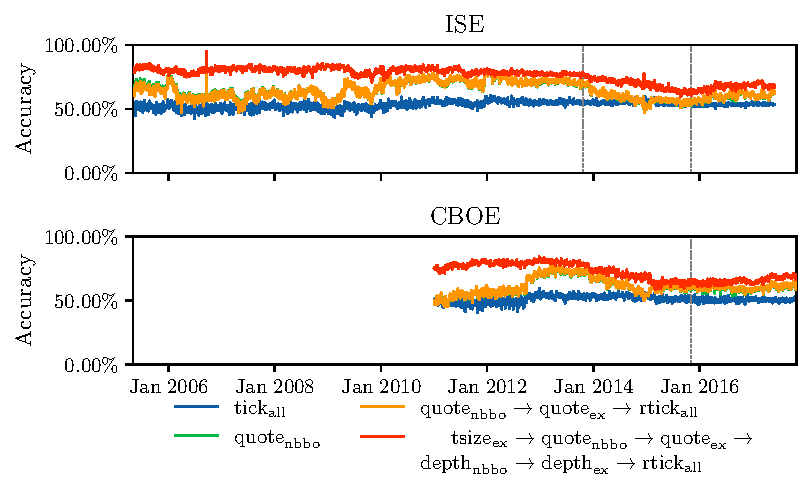
\includegraphics{classical-accuracies-over-time.pdf}
    \caption[Accuracy Of Rule-Based Classifiers On \glsentryshort{ISE} and \glsentryshort{CBOE} Over Time]{Accuracy of rule-based classifiers on \gls{ISE} and \gls{CBOE} sample over time. The dashed bar \myline{} indicates the beginning of a new subset based on the train-test split.}
    \label{fig:classical-accuracies-over-time}
\end{figure}

Aside from these high-level observations, we focus on three findings in greater detail.

\textbf{Finding 1: Accuracy of Tick-Based Algorithms Is Downward-Biased by Missingness}

\textbf{Finding 2: Accuracy Comes From Depth}

\textbf{Finding 3: Fee Structures Affect Accuracy Over Time}

\begin{table}[ht]
    \centering
    \caption[Accuracies of Rule-Based Approaches On \glsentryshort{CBOE}]{This table shows the accuracy of common trade classification rules and their variations for option trades on \gls{CBOE} sample. Unclassifiable trades by the respective rule are assigned randomly as buy or sell. Hybrid methods are estimated using trade prices across all exchanges. We report the percentage of classifiable trades and the overall accuracy for subsets based on our train-test split and the entire dataset. Best rule in \textbf{bold}.}
    \label{tab:cboe_supervised_all-master-cboe}
    \begin{tabular}{lSSSS}
        \toprule
        {}                                     & {Coverage in \%}  & \multicolumn{3}{c}{Accuracy in \%}                                         \\ \cmidrule(lr){2-2}\cmidrule(lr){3-5}
        {Trade Classification Rule}            & {All}             & {Pre-Test}                   & {Test}  & {All}             \\\midrule
        $\operatorname{tick}_{\mathrm{ex}}$    & 91.450            & 48.6156                            & 48.9969           & 48.7469           \\
        $\operatorname{rtick}_{\mathrm{ex}}$   & 90.280            & 51.0857                            & 50.5432           & 50.8989           \\
        $\operatorname{quote}_{\mathrm{ex}}$   & 94.460            & 62.6691                            & 62.0558           & 62.4580           \\
        $\operatorname{lr}_{\mathrm{ex}}$      & 99.850            & 62.4250                            & 61.7483           & 62.1921           \\
        $\operatorname{rlr}_{\mathrm{ex}}$     & 99.530            & 62.7111                            & 62.0071           & 62.4687           \\
        $\operatorname{emo}_{\mathrm{ex}}$     & 97.960            & 49.3923                            & 48.6489           & 49.1364           \\
        $\operatorname{remo}_{\mathrm{ex}}$    & 97.320            & 49.8883                            & 49.9529           & 49.9105           \\
        $\operatorname{clnv}_{\mathrm{ex}}$    & 98.440            & 54.2644                            & 53.2492           & 53.9149           \\
        $\operatorname{rclnv}_{\mathrm{ex}}$   & 94.040            & 55.1506                            & 54.5686           & 54.9502           \\\midrule
        $\operatorname{tick}_{\mathrm{all}}$   & 97.210            & 51.4199                            & 50.4403           & 51.0827           \\
        $\operatorname{rtick}_{\mathrm{all}}$  & 96.030            & 54.2521                            & 52.7056           & 53.7197           \\ \midrule
        $\operatorname{quote}_{\mathrm{nbbo}}$ & 94.770            & 61.3146                            & 59.7952           & 60.7915           \\
        $\operatorname{lr}_{\mathrm{nbbo}}$    & 99.870            & 61.0947                            & 59.5427           & 60.5604           \\
        $\operatorname{rlr}_{\mathrm{nbbo}}$   & 99.710            & 61.2959                            & 59.7516           & 60.7643           \\
        $\operatorname{emo}_{\mathrm{nbbo}}$   & 98.120            & 51.6420                            & 51.6299           & 51.6378           \\
        $\operatorname{remo}_{\mathrm{nbbo}}$  & 97.780            & 52.4847                            & 53.0735           & 52.6874           \\
        $\operatorname{clnv}_{\mathrm{nbbo}}$  & 98.540            & 55.3058                            & 54.1294           & 54.9008           \\
        $\operatorname{rclnv}_{\mathrm{nbbo}}$ & 98.350            & 56.3217                            & 55.4032           & 56.0055           \\\midrule
        $\operatorname{gsu}_{\mathrm{small}}$  & 99.780            & 61.6223                            & 60.3459           & 61.1829           \\
        $\operatorname{gsu}_{\mathrm{large}}$  & \bfseries 100.000 & \bfseries 73.8949                  & \bfseries 65.6943 & \bfseries 71.0717 \\\bottomrule
    \end{tabular}
\end{table}

We repeat the analysis on the \gls{CBOE} dataset in \cref{tab:cboe_supervised_all-master-cboe} and observe a similar ranking to \cref{tab:ise_supervised_all-master}. Overall, the performance of classical trade classification rules further diminishes strengthening the need for alternative classifiers. Tick-based rules trail the performance of quote-based approaches, and the accuracy of hybrids varies with the dependence on the tick test. Different from the \gls{ISE} sample, the quote rule estimated on the \gls{NBBO}, $\operatorname{quote}_{\mathrm{nbbo}}$, leads to a lower performance than the quote rule applied to \gls{CBOE} quotes. Parts of this is due to the fact, that  $\operatorname{quote}_{\mathrm{nbbo}}$ achieves a considerably lower coverage of \SI{94.77}{\percent} compared to \SI{99.89}{\percent} in the \gls{ISE} sample, with fewer trades classified by the fallback criterion. In a filtered common sample, where trades are classified by both rules, performance is approximately similar. Again, $\operatorname{gsu}_{\mathrm{small}}$ and $\operatorname{gsu}_{\mathrm{large}}$ perform best, the strong outperformance does not carry over to the test set \cref{fig:classical-accuracies-over-time}.\footnote{Performance on \gls{CBOE} can be improved if the order of quote rules is reversed. For full combinatoric coverage see \textcite[][33]{grauerOptionTradeClassification2022}. To avoid overfitting the test set by classical rules, we keep the baseline constant following our reasoning from \cref{sec:hyperparameter-tuning}.}

\todo{Doesn't this contradict the hidden order idea of Grauer?}

\begin{table}[H]
    \centering
    \caption[tbd]{tbd cboe}
    \label{tab:cboe_supervised_all-master-cboe}
    \begin{tabular}{lSSSS}
        \toprule
        {}                                                                                                                    & {Coverage in \%}  & \multicolumn{3}{c}{Accuracy in \%}                                         \\ \cmidrule(lr){2-2}\cmidrule(lr){3-5}
        {Trade Classification Rule}                                                                                           & {All}             & {Pre-Test}                         & {Test}            & {All}             \\\midrule
        $\operatorname{tick}_{\mathrm{all}}$                                                                                  & 97.210            & 51.4199                            & 50.4403           & 51.0827           \\
        $\operatorname{rtick}_{\mathrm{all}}$                                                                                 & 96.030            & 54.2521                            & 52.7056           & 53.7197           \\ \midrule
        $\operatorname{tick}_{\mathrm{ex}}$                                                                                   & 91.450            & 48.6156                            & 48.9969           & 48.7469           \\
        $\operatorname{rtick}_{\mathrm{ex}}$                                                                                  & 90.280            & 51.0857                            & 50.5432           & 50.8989           \\
        $\operatorname{quote}_{\mathrm{ex}}$                                                                                  & 94.460            & 62.6691                            & 62.0558           & 62.4580           \\
        $\operatorname{lr}_{\mathrm{ex}}$                                                                                     & 99.850            & 62.4250                            & 61.7483           & 62.1921           \\
        $\operatorname{rlr}_{\mathrm{ex}}$                                                                                    & 99.530            & 62.7111                            & 62.0071           & 62.4687           \\
        $\operatorname{emo}_{\mathrm{ex}}$                                                                                    & 97.960            & 49.3923                            & 48.6489           & 49.1364           \\
        $\operatorname{remo}_{\mathrm{ex}}$                                                                                   & 97.320            & 49.8883                            & 49.9529           & 49.9105           \\
        $\operatorname{clnv}_{\mathrm{ex}}$                                                                                   & 98.440            & 54.2644                            & 53.2492           & 53.9149           \\
        $\operatorname{rclnv}_{\mathrm{ex}}$                                                                                  & 94.040            & 55.1506                            & 54.5686           & 54.9502           \\\midrule
        $\operatorname{quote}_{\mathrm{nbbo}}$                                                                                & 94.770            & 61.3146                            & 59.7952           & 60.7915           \\
        $\operatorname{lr}_{\mathrm{nbbo}}$                                                                                   & 99.870            & 61.0947                            & 59.5427           & 60.5604           \\
        $\operatorname{rlr}_{\mathrm{nbbo}}$                                                                                  & 99.710            & 61.2959                            & 59.7516           & 60.7643           \\
        $\operatorname{emo}_{\mathrm{nbbo}}$                                                                                  & 98.120            & 51.6420                            & 51.6299           & 51.6378           \\
        $\operatorname{remo}_{\mathrm{nbbo}}$                                                                                 & 97.780            & 52.4847                            & 53.0735           & 52.6874           \\
        $\operatorname{clnv}_{\mathrm{nbbo}}$                                                                                 & 98.540            & 55.3058                            & 54.1294           & 54.9008           \\
        $\operatorname{rclnv}_{\mathrm{nbbo}}$                                                                                & 98.350            & 56.3217                            & 55.4032           & 56.0055           \\\midrule
        $\operatorname{quote}_{\mathrm{nbbo}} \to \operatorname{quote}_{\mathrm{ex}} \to \operatorname{rtick}_{\mathrm{all}}$ & 99.780            & 61.6223                            & 60.3459           & 61.1829           \\
        $\operatorname{gsu}$                                                                                                  & \bfseries 100.000 & \bfseries 73.8949                  & \bfseries 65.6943 & \bfseries 71.0717 \\\bottomrule
    \end{tabular}
\end{table}

\begin{figure}[ht]
    \centering
    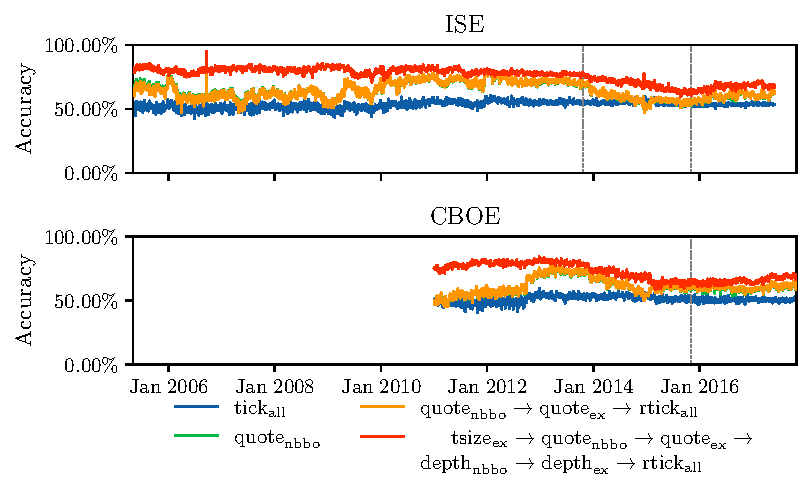
\includegraphics{classical-accuracies-over-time.pdf}
    \caption[tbd]{tbd.}
    \label{fig:classical-accuracies-over-time}
\end{figure}

\subsection{Results of Supervised
    Models}\label{sec:results-of-supervised-models}

Our models establish a new state-of-the-art for classification on the \gls{ISE} and \gls{CBOE} dataset, as we show.

\begin{figure}[ht]
    \centering
    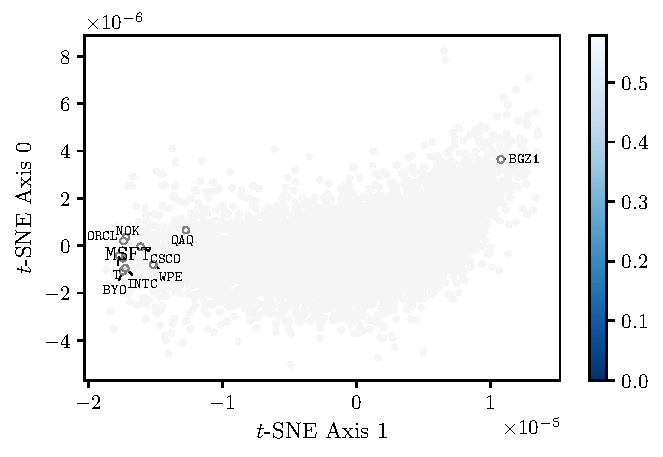
\includegraphics{categorical-embeddings.pdf}
    \caption[Categorical Embeddings of Underlyings]{Categorical embeddings of underlyings. The plot depicts the projected embedding of Microsoft ($\mathtt{MSFT}$) and its most similar embeddings. The similarity is highest for Intel ($\mathtt{INTC}$), Oracle ($\mathtt{ORCL}$), Nokia ($\mathtt{NOK}$), and Cisco ($\mathtt{CSCO}$). Embeddings are projected into 2D-space using $t$-SNE \autocite{vandermaatenVisualizingDataUsing2008}. The nine most similar embeddings by cosine similarity in the original space are coloured and annotated.}
    \label{fig:categorical-embeddings}
\end{figure}

\todo{Add more examples. Maybe also one with seldom class.
}

\subsection{Results of Semi-Supervised
    Models}\label{sec:results-of-semi-supervised-models}



\textbf{Gradient Boosting With Self-Training}

\textbf{FT-Transformer With Pretraining}

\subsection{Robustness of Results}\label{sec:robustness-checks}

\todo{Again, results are not 100 \% comparaable due to grouping.}
\todo{Compare improvements with other works. Improvments much greater than ronen et al. }

\textbf{Gradient Boosting}

\begin{table}[ht]
    \centering
    \caption[short-diff-ise-supervised-test-gbm]{long-diff-ise-supervised-test-gbm}
    \label{tab:diff-ise_supervised_test}
    \begin{tabular}{lSSSSSS@{}}
        \toprule
        {}                      & \multicolumn{2}{c}{FS Classical} & \multicolumn{2}{c}{FS Classical-Size} & \multicolumn{2}{c}{FS Option}                                        \\ \cmidrule(lr){2-3}\cmidrule(lr){4-5}\cmidrule(lr){6-7}
        {}                      & {Acc. in \%}                     & {Chg.}                                & {Acc. in \%}                  & {Chg.}    & {Acc. in \%} & {Chg.}    \\\midrule
        \multicolumn{7}{l}{ Option Type}                                                                                                                                          \\
        \tabindent C            & 62.890486                        & 3.930000                              & 71.884647                     & 4.890000  & 73.647971    & 6.650000  \\
        \tabindent P            & 64.557394                        & 3.720000                              & 72.867874                     & 5.430000  & 74.660185    & 7.220000  \\
        \cmidrule(rl){1-7}
        \multicolumn{7}{l}{ Security Type}                                                                                                                                        \\
        \tabindent Index option & 56.345043                        & -1.440000                             & 57.474458                     & -1.050000 & 58.649239    & 0.130000  \\
        \tabindent Others       & 68.399095                        & 3.080000                              & 76.369535                     & 6.230000  & 77.590573    & 7.450000  \\
        \tabindent Stock option & 61.877752                        & 4.210000                              & 70.946999                     & 4.800000  & 72.956919    & 6.810000  \\
        \cmidrule(rl){1-7}
        \multicolumn{7}{l}{ Trade Size}                                                                                                                                           \\
        \tabindent (0,1]        & 61.892029                        & 3.570000                              & 72.564793                     & 3.780000  & 74.245655    & 5.470000  \\
        \tabindent (1,3]        & 62.473959                        & 4.230000                              & 72.965377                     & 4.120000  & 74.857610    & 6.010000  \\
        \tabindent (3,5]        & 62.696932                        & 4.120000                              & 72.755628                     & 3.800000  & 74.647279    & 5.690000  \\
        \tabindent (5,11]       & 65.928967                        & 3.590000                              & 71.752039                     & 8.460000  & 73.450299    & 10.150000 \\
        \tabindent >11          & 67.310266                        & 3.840000                              & 71.337373                     & 6.790000  & 73.145472    & 8.600000  \\
        \cmidrule(rl){1-7}
        \multicolumn{7}{l}{ Year}                                                                                                                                                 \\
        \tabindent 2015         & 60.446922                        & 4.230000                              & 69.000296                     & 5.650000  & 71.512360    & 8.160000  \\
        \tabindent  2016        & 63.736474                        & 3.760000                              & 72.555638                     & 5.440000  & 74.290527    & 7.170000  \\
        \tabindent 2017         & 64.596306                        & 3.860000                              & 72.977560                     & 4.280000  & 74.604216    & 5.900000  \\
        \cmidrule(rl){1-7}
        \multicolumn{7}{l}{ Time To Maturity}                                                                                                                                     \\
        \tabindent <= 1         & 64.458297                        & 3.790000                              & 72.756774                     & 5.650000  & 74.604553    & 7.490000  \\
        \tabindent(1-2]         & 64.612677                        & 4.040000                              & 72.869099                     & 4.750000  & 73.947396    & 5.830000  \\
        \tabindent (2-3]        & 63.015912                        & 3.250000                              & 71.743691                     & 3.860000  & 72.997282    & 5.110000  \\
        \tabindent (3-6]        & 61.788369                        & 3.840000                              & 71.288086                     & 3.840000  & 72.750293    & 5.300000  \\
        \tabindent (6-12]       & 61.911555                        & 4.190000                              & 71.199996                     & 3.730000  & 73.130453    & 5.660000  \\
        \tabindent > 12         & 55.126547                        & 4.050000                              & 68.572852                     & 3.870000  & 72.004951    & 7.300000  \\
        \cmidrule(rl){1-7}
        \multicolumn{7}{l}{ Moneyness}                                                                                                                                            \\
        \tabindent <= 0.7       & 65.531247                        & 3.980000                              & 71.917341                     & 7.800000  & 72.307517    & 8.190000  \\
        \tabindent (0.7-0.9]    & 67.642270                        & 3.940000                              & 74.254665                     & 6.390000  & 75.433765    & 7.570000  \\
        \tabindent  (0.9-1.1]   & 64.059687                        & 3.750000                              & 72.975308                     & 4.820000  & 74.457482    & 6.310000  \\
        \tabindent (1.1-1.3]    & 54.294722                        & 4.160000                              & 66.220667                     & 4.560000  & 70.375579    & 8.720000  \\
        \tabindent > 1.3        & 52.623795                        & 3.790000                              & 63.075529                     & 3.100000  & 70.489510    & 10.510000 \\
        \cmidrule(rl){1-7}
        \multicolumn{7}{l}{ Proximity To Quotes}                                                                                                                                  \\
        \tabindent At Mid       & 62.644890                        & 5.950000                              & 72.164951                     & 6.260000  & 74.685118    & 8.780000  \\
        \tabindent Inside       & 62.605233                        & 2.400000                              & 68.301819                     & 4.060000  & 70.295127    & 6.050000  \\
        \tabindent At Quotes    & 67.828443                        & 7.860000                              & 86.667541                     & 8.450000  & 87.313763    & 9.100000  \\
        \tabindent Outside      & 61.350064                        & -5.420000                             & 61.846608                     & -3.050000 & 64.034087    & -0.860000 \\
        \tabindent Unknown      & 78.638385                        & 2.190000                              & 78.275744                     & 1.830000  & 78.816285    & 2.370000  \\
        \cmidrule(rl){1-7}
        \multicolumn{7}{l}{ All}                                                                                                                                                  \\
        \tabindent All          & 63.668637                        & 3.830000                              & 72.343640                     & 5.140000  & 74.120496    & 6.920000  \\
        \bottomrule
    \end{tabular}
\end{table}



\begin{table}[ht]
    \centering
    \caption[short-diff-cboe-transfer-test]{long-diff-cboe-gbm-tbd}
    \label{tab:diff-cboe_transfer-gbm}
    \begin{tabular}{lSSSSSS@{}}
        \toprule
        {}                      & \multicolumn{2}{c}{FS Classical} & \multicolumn{2}{c}{FS Classical-Size} & \multicolumn{2}{c}{FS Option}                                        \\ \cmidrule(lr){2-3}\cmidrule(lr){4-5}\cmidrule(lr){6-7}
        {}                      & {Acc. in \%}                     & {Chg.}                                & {Acc. in \%}                  & {Chg.}    & {Acc. in \%} & {Chg.}    \\\midrule
        \multicolumn{7}{l}{ Option Type}                                                                                                                                          \\
        \tabindent C            & 65.505083                        & 5.780000                              & 71.707057                     & 6.610000  & 74.283388    & 9.190000  \\
        \tabindent P            & 66.597419                        & 5.510000                              & 72.245014                     & 5.830000  & 74.484832    & 8.070000  \\
        \cmidrule(rl){1-7}
        \multicolumn{7}{l}{ Security Type}                                                                                                                                        \\
        \tabindent Index Option & 60.365562                        & 7.050000                              & 67.298912                     & 1.550000  & 72.394792    & 6.650000  \\
        \tabindent Others       & 69.054857                        & 4.860000                              & 74.137168                     & 6.080000  & 75.534837    & 7.470000  \\
        \tabindent Stock Option & 65.293961                        & 5.850000                              & 71.506273                     & 6.800000  & 74.089988    & 9.380000  \\
        \cmidrule(rl){1-7}
        \multicolumn{7}{l}{ Trade Size}                                                                                                                                           \\
        \tabindent (0,1]        & 62.831155                        & 6.200000                              & 70.756340                     & 7.500000  & 73.423543    & 10.160000 \\
        \tabindent (1,3]        & 64.895723                        & 5.590000                              & 71.318816                     & 7.130000  & 73.634574    & 9.450000  \\
        \tabindent (3,5]        & 65.549362                        & 5.500000                              & 71.956770                     & 6.500000  & 74.174579    & 8.720000  \\
        \tabindent(5,11]        & 66.577620                        & 5.630000                              & 71.566680                     & 6.090000  & 74.143799    & 8.670000  \\
        \tabindent >11          & 71.136074                        & 5.140000                              & 74.549126                     & 3.680000  & 76.765762    & 5.900000  \\
        \cmidrule(rl){1-7}
        \multicolumn{7}{l}{ Year}                                                                                                                                                 \\
        \tabindent 2015         & 65.689585                        & 4.850000                              & 71.445193                     & 7.340000  & 74.317847    & 10.220000 \\
        \tabindent 2016         & 65.579978                        & 5.770000                              & 71.638148                     & 7.290000  & 74.178699    & 9.830000  \\
        \tabindent 2017         & 66.491658                        & 5.640000                              & 72.349451                     & 5.020000  & 74.591947    & 7.260000  \\
        \cmidrule(rl){1-7}
        \multicolumn{7}{l}{ Time To Maturity}                                                                                                                                     \\
        \tabindent <= 1         & 66.863272                        & 5.410000                              & 72.005520                     & 6.020000  & 74.272153    & 8.290000  \\
        \tabindent (1-2]        & 67.553775                        & 5.950000                              & 72.584599                     & 5.990000  & 75.237684    & 8.640000  \\
        \tabindent (2-3]        & 66.061857                        & 6.080000                              & 72.349461                     & 5.930000  & 74.713903    & 8.300000  \\
        \tabindent(3-6]         & 65.007308                        & 6.250000                              & 72.855935                     & 7.020000  & 75.086134    & 9.250000  \\
        \tabindent(6-12]        & 64.184403                        & 5.890000                              & 71.908786                     & 6.870000  & 74.389885    & 9.360000  \\
        \tabindent > 12         & 56.065976                        & 5.580000                              & 66.802260                     & 7.580000  & 71.092148    & 11.870000 \\
        \cmidrule(rl){1-7}
        \multicolumn{7}{l}{ Moneyness}                                                                                                                                            \\
        \tabindent <= 0.7       & 65.722320                        & 5.740000                              & 72.842929                     & 4.820000  & 75.645703    & 7.630000  \\
        \tabindent (0.7-0.9]    & 66.272446                        & 5.900000                              & 72.187575                     & 5.980000  & 74.768887    & 8.570000  \\
        \tabindent (0.9-1.1]    & 66.977290                        & 5.610000                              & 72.619255                     & 6.260000  & 74.739508    & 8.380000  \\
        \tabindent (1.1-1.3]    & 58.197013                        & 5.190000                              & 66.153817                     & 7.660000  & 69.833429    & 11.340000 \\
        \tabindent > 1.3        & 56.958403                        & 6.070000                              & 64.569317                     & 7.220000  & 70.478616    & 13.130000 \\
        \cmidrule(rl){1-7}
        \multicolumn{7}{l}{ Proximity To Quotes}                                                                                                                                  \\
        \tabindent At Mid       & 60.997665                        & 7.130000                              & 67.848014                     & 8.490000  & 69.845251    & 10.490000 \\
        \tabindent Inside       & 68.822448                        & 3.580000                              & 71.987785                     & 6.680000  & 73.698272    & 8.390000  \\
        \tabindent At Quotes    & 54.187224                        & 16.010000                             & 74.756821                     & 2.410000  & 81.426352    & 9.080000  \\
        \tabindent Outside      & 70.719978                        & -4.170000                             & 70.369607                     & -1.550000 & 69.648255    & -2.270000 \\
        \tabindent Unknown      & 83.771336                        & 1.130000                              & 83.608778                     & 0.970000  & 84.213854    & 1.570000  \\
        \cmidrule(rl){1-7}
        \multicolumn{7}{l}{ All}                                                                                                                                                  \\
        \tabindent All          & 66.002029                        & 5.660000                              & 71.951794                     & 6.260000  & 74.375033    & 8.680000  \\
        \bottomrule
    \end{tabular}
\end{table}


\textbf{FT-Transformer}

\begin{table}[ht]
    \centering
    \caption[short-diff-ise-supervised-test-fttransformer]{long-diff-ise-supervised-test-fttransformer}
    \label{tab:diff-ise_supervised-test}
    \begin{tabular}{lSSSSSS@{}}
        \toprule
        {}                      & \multicolumn{2}{c}{FS Classical} & \multicolumn{2}{c}{FS Classical-Size} & \multicolumn{2}{c}{FS Option}                                        \\ \cmidrule(lr){2-3}\cmidrule(lr){4-5}\cmidrule(lr){6-7}
        {}                      & {Acc. in \%}                     & {Chg.}                                & {Acc. in \%}                  & {Chg.}    & {Acc. in \%} & {Chg.}    \\\midrule
        \multicolumn{7}{l}{ Option Type}                                                                                                                                          \\
        \tabindent C            & 62.991514                        & 4.030000                              & 72.099064                     & 5.100000  & 73.484904    & 6.490000  \\
        \tabindent P            & 64.687031                        & 3.840000                              & 73.131667                     & 5.690000  & 74.420786    & 6.980000  \\
        \cmidrule(rl){1-7}
        \multicolumn{7}{l}{ Security Type}                                                                                                                                        \\
        \tabindent Index option & 56.519890                        & -1.260000                             & 58.457380                     & -0.070000 & 58.641678    & 0.120000  \\
        \tabindent Others       & 68.443599                        & 3.120000                              & 76.549050                     & 6.410000  & 77.590109    & 7.450000  \\
        \tabindent Stock option & 62.019384                        & 4.350000                              & 71.196166                     & 5.050000  & 72.674763    & 6.520000  \\
        \cmidrule(rl){1-7}
        \multicolumn{7}{l}{ Trade Size}                                                                                                                                           \\
        \tabindent (0,1]        & 62.127137                        & 3.800000                              & 72.877007                     & 4.100000  & 73.967386    & 5.190000  \\
        \tabindent(1,3]         & 62.654716                        & 4.410000                              & 73.321548                     & 4.480000  & 74.721308    & 5.880000  \\
        \tabindent (3,5]        & 62.839285                        & 4.270000                              & 73.161769                     & 4.200000  & 74.715927    & 5.760000  \\
        \tabindent (5,11]       & 65.756057                        & 3.410000                              & 71.877263                     & 8.580000  & 73.441354    & 10.150000 \\
        \tabindent >11          & 67.380602                        & 3.910000                              & 71.237293                     & 6.690000  & 72.584805    & 8.040000  \\
        \cmidrule(rl){1-7}
        \multicolumn{7}{l}{ Year}                                                                                                                                                 \\
        \tabindent 2015         & 60.620179                        & 4.410000                              & 69.609946                     & 6.260000  & 71.861077    & 8.510000  \\
        \tabindent 2016         & 63.851905                        & 3.870000                              & 72.798245                     & 5.680000  & 74.138951    & 7.020000  \\
        \tabindent 2017         & 64.688426                        & 3.950000                              & 73.077731                     & 4.380000  & 74.111711    & 5.410000  \\
        \cmidrule(rl){1-7}
        \multicolumn{7}{l}{ Time To Maturity}                                                                                                                                     \\
        \tabindent <= 1         & 64.546416                        & 3.880000                              & 72.976628                     & 5.860000  & 74.450445    & 7.340000  \\
        \tabindent(1-2]         & 64.736461                        & 4.170000                              & 73.043470                     & 4.930000  & 73.692560    & 5.570000  \\
        \tabindent (2-3]        & 63.152545                        & 3.380000                              & 72.063690                     & 4.180000  & 72.896064    & 5.010000  \\
        \tabindent (3-6]        & 61.887659                        & 3.940000                              & 71.531191                     & 4.080000  & 72.287641    & 4.830000  \\
        \tabindent (6-12]       & 62.021518                        & 4.300000                              & 71.325950                     & 3.860000  & 72.466903    & 5.000000  \\
        \tabindent > 12         & 55.669126                        & 4.590000                              & 69.313656                     & 4.610000  & 72.282466    & 7.580000  \\
        \cmidrule(rl){1-7}
        \multicolumn{7}{l}{ Moneyness}                                                                                                                                            \\
        \tabindent <= 0.7       & 65.196444                        & 3.650000                              & 71.762641                     & 7.650000  & 71.689001    & 7.580000  \\
        \tabindent (0.7-0.9]    & 67.618182                        & 3.910000                              & 74.318808                     & 6.450000  & 74.876535    & 7.010000  \\
        \tabindent (0.9-1.1]    & 64.141472                        & 3.830000                              & 73.115683                     & 4.960000  & 74.236648    & 6.080000  \\
        \tabindent (1.1-1.3]    & 54.943206                        & 4.810000                              & 67.505754                     & 5.850000  & 70.929706    & 9.270000  \\
        \tabindent > 1.3        & 53.468351                        & 4.630000                              & 64.293219                     & 4.320000  & 71.424038    & 11.450000 \\
        \cmidrule(rl){1-7}
        \multicolumn{7}{l}{ Proximity To Quotes}                                                                                                                                  \\
        \tabindent At Mid       & 62.490146                        & 5.790000                              & 72.138236                     & 6.230000  & 74.022892    & 8.120000  \\
        \tabindent Inside       & 62.566010                        & 2.360000                              & 68.807735                     & 4.560000  & 70.429973    & 6.190000  \\
        \tabindent At Quotes    & 68.608870                        & 8.640000                              & 86.087938                     & 7.870000  & 86.165327    & 7.950000  \\
        \tabindent Outside      & 63.228880                        & -3.540000                             & 63.792525                     & -1.100000 & 65.610951    & 0.720000  \\
        \tabindent Unknown      & 78.268902                        & 1.820000                              & 77.824153                     & 1.380000  & 78.522066    & 2.070000  \\
        \cmidrule(rl){1-7}
        \multicolumn{7}{l}{ All}                                                                                                                                                  \\
        \tabindent All          & 63.783020                        & 3.940000                              & 72.581107                     & 5.380000  & 73.921795    & 6.720000  \\
        \bottomrule
    \end{tabular}
\end{table}

\begin{table}[ht]
    \centering
    \caption[short-diff-cboe-transfer-test-fttransformer]{long-diff-cboe-transfer-test-fttransformer}
    \label{tab:diff-cboe_transfer_test}
    \begin{tabular}{lSSSSSS@{}}
        \toprule
        {}                      & \multicolumn{2}{c}{FS Classical} & \multicolumn{2}{c}{FS Classical-Size} & \multicolumn{2}{c}{FS Option}                                       \\ \cmidrule(lr){2-3}\cmidrule(lr){4-5}\cmidrule(lr){6-7}
        {}                      & {Acc. in \%}                     & {Chg.}                                & {Acc. in \%}                  & {Chg.}   & {Acc. in \%} & {Chg.}    \\\midrule
        \multicolumn{7}{l}{ Option Type}                                                                                                                                         \\
        \tabindent C            & 65.628907                        & 5.900000                              & 71.945453                     & 6.850000 & 74.579113    & 9.480000  \\
        \tabindent P            & 66.845425                        & 5.760000                              & 72.402406                     & 5.990000 & 73.917935    & 7.510000  \\
        \cmidrule(rl){1-7}
        \multicolumn{7}{l}{ Security Type}                                                                                                                                       \\
        \tabindent Index option & 61.207800                        & 7.890000                              & 67.170125                     & 1.420000 & 69.051358    & 3.310000  \\
        \tabindent Others       & 69.266211                        & 5.070000                              & 74.427252                     & 6.370000 & 75.859396    & 7.800000  \\
        \tabindent Stock option & 65.395694                        & 5.950000                              & 71.703855                     & 7.000000 & 74.141068    & 9.430000  \\
        \cmidrule(rl){1-7}
        \multicolumn{7}{l}{ Trade Size}                                                                                                                                          \\
        \tabindent (0,1]        & 63.135782                        & 6.500000                              & 71.074930                     & 7.820000 & 73.362654    & 10.100000 \\
        \tabindent (1,3]        & 64.993995                        & 5.690000                              & 71.513064                     & 7.330000 & 73.846381    & 9.660000  \\
        \tabindent (3,5]        & 65.605000                        & 5.560000                              & 72.070498                     & 6.610000 & 74.237799    & 8.780000  \\
        \tabindent (5,11]       & 66.701471                        & 5.750000                              & 71.890991                     & 6.420000 & 73.979636    & 8.510000  \\
        \tabindent >11          & 71.378727                        & 5.380000                              & 74.552019                     & 3.680000 & 76.246445    & 5.380000  \\
        \cmidrule(rl){1-7}
        \multicolumn{7}{l}{ Year}                                                                                                                                                \\
        \tabindent 2015         & 65.830149                        & 4.990000                              & 71.843643                     & 7.740000 & 74.755266    & 10.650000 \\
        \tabindent 2016         & 65.786999                        & 5.970000                              & 71.935076                     & 7.590000 & 74.353864    & 10.010000 \\
        \tabindent 2017         & 66.648330                        & 5.790000                              & 72.424788                     & 5.090000 & 74.138831    & 6.810000  \\
        \cmidrule(rl){1-7}
        \multicolumn{7}{l}{ Time To Maturity}                                                                                                                                    \\
        \tabindent<= 1          & 66.927563                        & 5.470000                              & 72.081695                     & 6.100000 & 74.167407    & 8.180000  \\
        \tabindent(1-2]         & 67.642166                        & 6.040000                              & 72.576488                     & 5.980000 & 74.914699    & 8.320000  \\
        \tabindent (2-3]        & 66.550561                        & 6.570000                              & 72.383470                     & 5.970000 & 73.512089    & 7.100000  \\
        \tabindent (3-6]        & 65.257500                        & 6.500000                              & 73.243404                     & 7.410000 & 75.241041    & 9.410000  \\
        \tabindent (6-12]       & 64.630833                        & 6.330000                              & 72.430785                     & 7.400000 & 74.759232    & 9.720000  \\
        \tabindent > 12         & 56.949258                        & 6.460000                              & 68.451314                     & 9.230000 & 71.975430    & 12.760000 \\
        \cmidrule(rl){1-7}
        \multicolumn{7}{l}{ Moneyness}                                                                                                                                           \\
        \tabindent <= 0.7       & 65.747181                        & 5.770000                              & 72.938769                     & 4.920000 & 75.030310    & 7.010000  \\
        \tabindent (0.7-0.9]    & 66.501088                        & 6.130000                              & 72.160406                     & 5.960000 & 73.928341    & 7.730000  \\
        \tabindent (0.9-1.1]    & 67.105536                        & 5.740000                              & 72.698844                     & 6.340000 & 74.754866    & 8.400000  \\
        \tabindent (1.1-1.3]    & 58.732468                        & 5.720000                              & 67.827369                     & 9.340000 & 70.847531    & 12.360000 \\
        \tabindent > 1.3        & 57.597394                        & 6.700000                              & 66.397443                     & 9.050000 & 71.088957    & 13.740000 \\
        \cmidrule(rl){1-7}
        \multicolumn{7}{l}{ Proximity To Quotes}                                                                                                                                 \\
        \tabindent At Mid       & 60.688727                        & 6.820000                              & 67.528635                     & 8.170000 & 69.104800    & 9.750000  \\
        \tabindent Inside       & 68.679525                        & 3.440000                              & 72.284311                     & 6.970000 & 73.930387    & 8.620000  \\
        \tabindent At Quotes    & 56.479734                        & 18.300000                             & 74.815580                     & 2.470000 & 79.999142    & 7.650000  \\
        \tabindent Outside      & 73.145095                        & -1.740000                             & 72.581753                     & 0.660000 & 71.908491    & -0.010000 \\
        \tabindent Unknown      & 83.807460                        & 1.160000                              & 83.220446                     & 0.580000 & 83.491375    & 0.850000  \\
        \cmidrule(rl){1-7}
        \multicolumn{7}{l}{ All}                                                                                                                                                 \\
        \tabindent All          & 66.182348                        & 5.840000                              & 72.153338                     & 6.460000 & 74.278318    & 8.580000  \\
        \bottomrule
    \end{tabular}
\end{table}

\todo{When the analysis was repeated using only the Lee and Radhakrishna subsample, the results were equally as strong or stronger, with two exceptions. Using their subsample, time between transactions is no longer a statistically signi"cant determinant of misclassi"cation and large trades are misclassi"ed slightly more frequently than small trades (odderswhite)}
\todo{Our focus is on ... rules.}
\todo{Improvements are particularily high for trades that are notourisly hard to classify by classical trade classification algorithms.}

\subsection{Feature Importance}\label{sec:feature-importance}

\newpage
\section{Application in Transaction Cost Estimation}\label{sec:application}

\textbf{Preliminaries}

% TODO: Add why it is important. See Stoll, Huang, Roll (zettelkasten)

Albeit the classification accuracy is a reasonable measure for comparing classifiers, one cannot immediately infer how changes in accuracy e.~g., an improvement by \SI{1}{\percent}, affect the application domains. In an attempt to make our results tangible, we apply all algorithms to estimate trading cost, a problem we previously identified to be reliant on correct trade classification (cp. \cref{sec:introduction}) and a common testing ground for trade classification rules \autocites[cp.][541]{ellisAccuracyTradeClassification2000}[][569]{finucaneDirectTestMethods2000}[][271--278]{petersonEvaluationBiasesExecution2003}[][896--897]{savickasInferringDirectionOption2003}.

One of the most widely adopted measures for trading costs is the effective spread \autocite[][112]{Piwowar_2006}. It is defined as the difference between the trade price and the fundamental value of the asset \autocite[][238--239]{bessembinderIssuesAssessingTrade2003}. Following \textcite[][238--239]{bessembinderIssuesAssessingTrade2003}, we define the \emph{nominal, effective spread} as
\begin{equation}
    S_{i,t} = 2 (P_{i,t} - V_{i,t}) D_{i,t}.
    \label{eq:effective-spread}
\end{equation}

Like before, $i$ indexes the security and $t$ the point in time. Here, $D_{i,t}$ is the trade direction, which is either $1$ for customer buy orders and $-1$ for sell orders. If the trade initiator is known, we set $D_{i,t} = y_{i,t}$ and $D_{i,t}=\hat{y}_{it}$, if inferred from a rule or classifier. As the fundamental value $V_{i,t}$ is unobserved at the time of the trade, we follow a common track in research and use the midpoint of the prevailing quotes as an observable proxy.\footnote{An alternative treatment for options is discussed in \textcite[][4975--4976]{muravyevOptionsTradingCosts2020} Our focus is on the midspread, as it is the most common proxy for the value.} This is also a natural choice, under the assumption that, on average, the spread is symmetric and centred around the true fundamental value \autocite[][1018]{leeMarketIntegrationPrice1993}. We multiply the so-obtained half-spread by $\times 2$ to obtain the effective spread, which represents the cost for a round trip trade involving a buy and sell excluding commissions.

Apparent from \cref{eq:effective-spread}, poor estimates for the predicted trade direction, lead to an under or overestimated effective spread, and hence to a skewed trade cost estimate. Only for trades at the midspread, the predicted trade direction is irrelevant, since the effective spread is zero. By comparing the true effective spread from the estimated, we can derive the economic significance. For convenience, we also calculate the \emph{relative effective spread} as
\begin{equation}
    {PS}_{i,t} = S_{i,t} / V_{i,t}.
\end{equation}
% FIXME: check how it is defined Savickas / Finucane use midpoint, Peterson and Sirri divide by price / so does chakrabarty 2007 p. 3819?
The subsequent section estimates both the nominal and relative effective spread for our test sets, as well as the quoted spread.

\textbf{Results}

The actual and the estimated effective spreads, as well as the quoted spread, are shown in the \cref{tab:effective-spread} aggregated by mean. \textcite[][896--897]{savickasInferringDirectionOption2003} estimated the effective spreads on a subset of rules for option trades at the \gls{CBOE}, which can be compared against.

\begin{table}[H]
    \centering
    \begin{threeparttable}
    \sisetup{
        round-precision = 3, 
      }
    \begin{tabular}{llSSSS}
        \toprule
        {}                                               & {}   & \multicolumn{2}{c}{\gls{ISE}} & \multicolumn{2}{c}{\gls{CBOE}}                                 \\ \cmidrule(lr){3-4}\cmidrule(lr){5-6}
        {Classifier}                                     & {FS} & {Dollar}                      & {Relative}                     & {Dollar} & {Relative}         \\ \midrule
        \multicolumn{6}{l}{Rule-Based}                                                                                                                           \\
        \tabindent $\operatorname{tick}_{\mathrm{ex}}$   & 1    & 0.015534                      & 0.010777 \tnote{*}             & 0.014179 & 0.022880 \tnote{*} \\
        \tabindent $\operatorname{quote}_{\mathrm{ex}}$  & 1    & 0.163333                      & 0.162074 \tnote{*}             & 0.125388 & 0.142093 \tnote{*} \\
        \tabindent $\operatorname{lr}_{\mathrm{ex}}$     & 1    & 0.163333                      & 0.162074 \tnote{*}             & 0.125388 & 0.142093 \tnote{*} \\
        \tabindent $\operatorname{emo}_{\mathrm{ex}}$    & 1    & 0.046443                      & 0.084442 \tnote{*}             & 0.041138 & 0.074176 \tnote{*} \\ 
        \tabindent $\operatorname{clnv}_{\mathrm{ex}}$   & 1    & 0.116247                      & 0.132842 \tnote{*}             & 0.086715 & 0.110510 \tnote{*} \\ 
        \tabindent $\operatorname{gsu}_{\mathrm{small}}$ & 2    & 0.065670                      & 0.096277 \tnote{*}             & 0.084145 & 0.107195 \tnote{*} \\
        \tabindent $\operatorname{gsu}_{\mathrm{large}}$ & 2    & 0.016734                      & 0.044854 \tnote{*}             & 0.053114 & 0.072212 \tnote{*} \\ \midrule
        \multicolumn{6}{l}{Supervised}                                                                                                                           \\
        \tabindent \gls{GBRT}                            & 1    & 0.074294                      & 0.091619 \tnote{*}             & 0.060933 & 0.095318 \tnote{*} \\
        \tabindent \gls{GBRT}                            & 2    & 0.042556                      & 0.069838 \tnote{*}             & 0.036213 & 0.071433 \tnote{*} \\
        \tabindent \gls{GBRT}                            & 3    & 0.039437                      & 0.066473 \tnote{*}             & 0.034674 & 0.066758 \tnote{*} \\ 
        \tabindent  FT-Transformer                       & 2    & 0.030291                      & 0.065596 \tnote{*}             & 0.024942 & 0.063574 \tnote{*} \\
        \tabindent  FT-Transformer                       & 1    & 0.065871                      & 0.086339 \tnote{*}             & 0.057153 & 0.090205 \tnote{*} \\
        \tabindent  FT-Transformer                       & 3    & 0.029874                      & 0.063486 \tnote{*}             & 0.021487 & 0.057358 \tnote{*} \\ \midrule
        \multicolumn{6}{l}{Semi-Supervised}                                                                                                                      \\
        \tabindent \gls{GBRT}                            & 1    & 0.075724                      & 0.092439 \tnote{*}             & 0.065420 & 0.096814 \tnote{*} \\
        \tabindent \gls{GBRT}                            & 2    & 0.043359                      & 0.072062 \tnote{*}             & 0.039600 & 0.073760 \tnote{*} \\
        \tabindent \gls{GBRT}                            & 3    & 0.043240                      & 0.069230 \tnote{*}             & 0.037083 & 0.067946 \tnote{*} \\ 
        \tabindent  FT-Transformer                       & 1    &                               & \tnote{*}                      &          & \tnote{*}          \\
        \tabindent  FT-Transformer                       & 2    &                               & \tnote{*}                      &          & \tnote{*}          \\
        \tabindent  FT-Transformer                       & 3    &                               & \tnote{*}                      &          & \tnote{*}          \\ \midrule
        True Effective Spread                            &      & 0.004926                      & 0.037159                       & 0.012219 & 0.025122           \\ \bottomrule
        % Quoted Spread                                    &      &                                                   &                                                    &          &                 \\ \bottomrule
    \end{tabular}
    \begin{tablenotes}\footnotesize
        \item[*] $p \leq 0.01$.
    \end{tablenotes}
\end{threeparttable}
    \caption{Effective Spreads Estimates of Trade Classification Rules and Classifiers}
    \label{tab:effective-spread}
\end{table}

Following \textcite[][12]{theissenTestAccuracyLee2000} a Wilcoxon test is conducted to assess if the medians of the estimated, effective spread and the true effective spread are equal. The null hypothesis of equal medians is rejected for $p \leq 0.01$.

\todo{Seems to be standard procedure to exclude some trades due to illiquidity. Could heal the problem with very large spreads \url{https://derivate.fbv.kit.edu/download/Eberbach_Uhrig-Homburg_Yu_2021.pdf}}

% TODO: Discuss results. See Zettelkasten.